
\subsection{Gadget Construction}

An \emph{$\mathcal F$-gate} is a finite signature grid over $\mathcal F$
with some dangling edges; summing over its internal edges realizes the
signature on the dangling edges. 
%We say a signature $f$ is \emph{realizable} from $\F$, if $\Holant(\F,f)\leq_T \Holant(\F)$.
It is clear that if $f$ is the signature of an $\mathcal F$-gate, it is realizable from $\mathcal{F}.$
In the following we do not distinguish an $\mathcal{F}$-gate and its signature.

We record some frequently used gadgets in this paper. 
The following four basic constructions are illustrated in \cref{fig:gadget-constructions}.

\paragraph{Merging}
Given a binary signature $b$ and a signature $f$ with distinct variables $x_i,x_j$, the signature obtained \emph{merging} (or \emph{contracting}) variables $x_i,x_j$ of $f$ using $b$ is the following signature
\[
(\partial_{ij}^b f)(x_{[n]\setminus\{i,j\}})
=\sum_{a,c\in\{0,1\}}b(a,c)
  f(x_1,\ldots,x_{i-1},a,x_{i+1},\ldots,x_{j-1},c,x_{j+1},\ldots,x_n).
\]
When $b$ is $=_2$, we simply say merge $x_i$ and $x_j$ of $f$. 
We abbreviate
$\partial_{ij}f:=\partial_{ij}^{=_2}f=f_{ij}^{00}+f_{ij}^{11}$.
We also use the notation $\partial^{M(b)}_{ij}f$ for $\partial^{b}_{ij}f$, where $M(b)$ is the $2$ by 2 signature matrix of $b$.
We use $\partial_{(i_1j_1)\ldots(i_kj_k)}f$ to denote $\partial_{i_1j_1}\ldots\partial_{i_kj_k}f$ for short.
It is clear that the operators $\partial_{ij}$ and $\partial_{k\ell}$ commute if $\{i,j\}\cap \{k,\ell\}=\emptyset.$
For a signature class $\mathscr C$, the notation
$f\in\int\mathscr C$ means that
$\partial_{ij}f\in\mathscr C$ for every pair $i\ne j$.

\paragraph{Binary extension}
    Given a binary signature $b(x_1,x_2)$ and an arity-$n$ signature $f(y_1,\ldots, y_n)$, we may connect $x_i$ of $b$ to $y_j$ of $f$, and obtain a new signature.
    This is called a \emph{binary extension} or \emph{binary modification} to $f$.



\begin{lemma}\label{lem-binary-sim}
    Let ${b_1}(x_1, y_1), {b_2}(x_2, y_2)\in {\mathcal{U}}$. 
    If by connecting the variable $x_1$ of ${b_1}$ and the variable $x_2$ of ${b_2}$ using $=_2$, we get $\lambda\cdot (=_2)(y_1, y_2)$ for some $\lambda\in \mathbb{C}^\times$, then ${b_1}\sim \overline{b_2}$. 
    Moreover, by connecting the variable $y_1$ of ${b_1}$ and the variable $y_2$ of ${b_2}$, we will get $\lambda\cdot (=_2)(x_1, x_2)$.
\end{lemma}

\begin{proof}
Clearly both $b_1$ and $b_2$ are non-zero, otherwise connecting them we obtain a zero signature.
Since $b_1, b_2\in \mathcal{U}$ and they are non-zero, there exists $\lambda_1,\lambda_2\in \mathbb C^\times$ such that $M(b_1)M(b_1)^\dagger=\lambda_1I_2$ and  $M(b_2)M(b_2)^\dagger=\lambda_2I_2$.
%Consider matrices $M_1(b_1)=M^{\tt T}_2(b_1)$ and $M_1(b_2)=M^{\tt T}_2(b_2)$.
By connecting $x_1$ of $b_1$ and $x_2$ of $b_2$, we obtain the binary signature $b_3(y_1,y_2)$ with matrix $M(b_3)=M(b_1)^{\tt T}M(b_2)=\lambda I_2$ for some $\lambda\in \mathbb{C}^\times.$
So $M(b_2)=\lambda (M(b_1)^{\tt T})^{-1}=\frac{\lambda}{\lambda_1} \overline{M(b_1)}$.
Hence $b_1\sim \overline{b_2}$.
Also, by connecting the variable $y_1$ of ${b_1}$ and the variable $y_2$ of ${b_2}$, we will get the signature $b_4(x_1,x_2)$ with matrix $M(b_4)=M(b_1)M(b_2)^{\tt T}=M(b_1)\cdot \frac{\lambda}{\lambda_1}M(b_1)^\dagger=\lambda\cdot(=_2)(x_1, x_2).$
\end{proof}

\paragraph{Mating and first order orthogonality}
Given a (complex-valued) signature $f$ of arity $n\geqslant 2$, we connect $f$ and $\overline{f}$ in the following manner:
Fix a set $S$ of $n-m$ variables among all $n$ variables of $f$. 
For each $x_k\in S$, connect $x_k$ of $f$ with the corresponding variable $x_k$ of $\overline{f}$ using $=_2$. 
The variables that are not in $S$ are called dangling variables.
%In this paper, we only consider the case that $m=1$ or $2$.
For $m=1$, there is one dangling variable $x_i$. Then, 
the mating construction  realizes a binary signature, denoted by $\mathfrak m_{i}f$.
\begin{figure}[t]
\centering
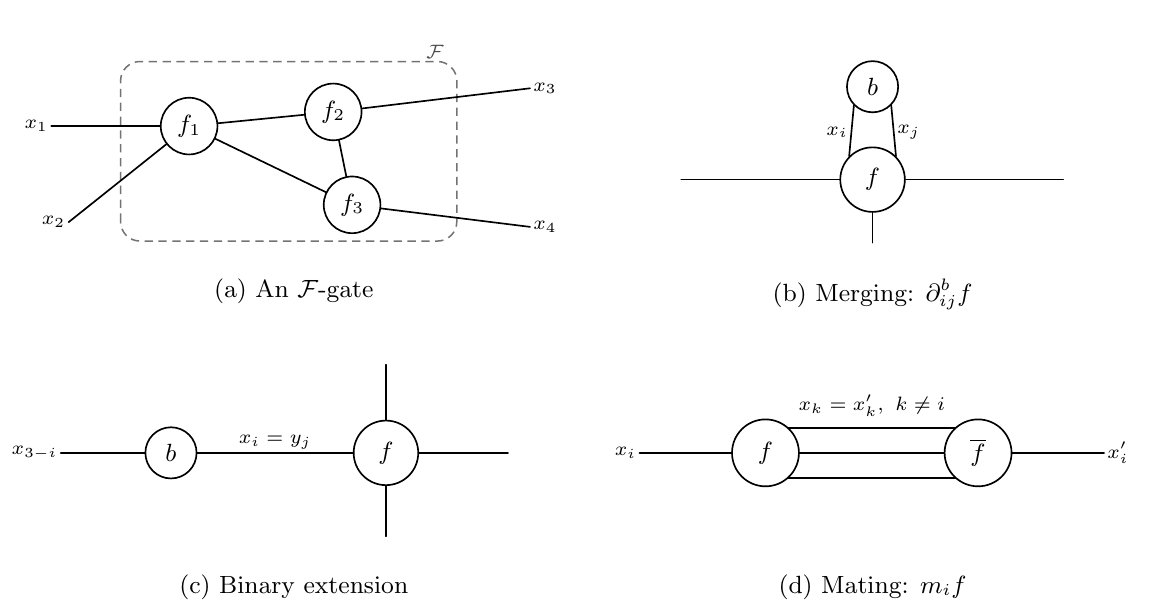
\begin{tikzpicture}[
    wire/.style={draw=black, line width=0.6pt, line cap=round},
    boundary/.style={draw=black!55, densely dashed, line width=0.55pt,
        rounded corners=7pt},
    signature/.style={draw=black, circle, fill=white, minimum size=7.2mm,
        inner sep=0pt, line width=0.6pt, font=\small},
    small signature/.style={signature, minimum size=6.5mm},
    port label/.style={font=\scriptsize, inner sep=1pt},
    panel label/.style={font=\small, anchor=north}
]

% (a) An F-gate
\begin{scope}[shift={(0,3.75)}]
    \path[use as bounding box] (0,0) rectangle (6.75,3.35);

    \draw[boundary] (1.18,0.64) rectangle (5.45,2.92);
    \node[port label, anchor=south east, text=black!70]
        at (5.33,2.92) {$\mathcal F$};

    \draw[wire] (0.30,2.10) -- (2.05,2.10);
    \draw[wire] (0.52,0.88) -- (2.05,2.10);
    \draw[wire] (2.05,2.10) -- (3.88,2.28);
    \draw[wire] (2.05,2.10) -- (4.12,1.10);
    \draw[wire] (3.88,2.28) -- (4.12,1.10);
    \draw[wire] (3.88,2.28) -- (6.38,2.58);
    \draw[wire] (4.12,1.10) -- (6.38,0.82);

    \node[signature] at (2.05,2.10) {$f_1$};
    \node[signature] at (3.88,2.28) {$f_2$};
    \node[signature] at (4.12,1.10) {$f_3$};

    \node[port label, left] at (0.30,2.10) {$x_1$};
    \node[port label, left] at (0.52,0.88) {$x_2$};
    \node[port label, right] at (6.38,2.58) {$x_3$};
    \node[port label, right] at (6.38,0.82) {$x_4$};
    \node[panel label] at (3.38,0.28)
        {\textup{(a)} An $\mathcal F$-gate};
\end{scope}

% (b) Merging two variables of f using b
\begin{scope}[shift={(7.35,3.75)}]
    \path[use as bounding box] (0,0) rectangle (6.75,3.35);

    \node[small signature] (merge-b) at (3.38,2.60) {$b$};
    \node[signature, minimum size=8.2mm] (merge-f) at (3.38,1.42) {$f$};

    \draw[wire] (merge-b.225) --
        node[port label, left, pos=0.53] {$x_i$} (merge-f.135);
    \draw[wire] (merge-b.315) --
        node[port label, right, pos=0.53] {$x_j$} (merge-f.45);
    \draw[wire] (0.95,1.42) -- (merge-f.180);
    \draw[wire] (merge-f.0) -- (5.80,1.42);
    \draw[wire] (3.38,0.62) -- (merge-f.270);

    \node[panel label] at (3.38,0.28)
        {\textup{(b)} Merging: $\partial_{ij}^{b}f$};
\end{scope}

% (c) Binary extension
\begin{scope}
    \path[use as bounding box] (0,0) rectangle (6.75,3.35);

    \node[small signature] (ext-b) at (1.82,1.70) {$b$};
    \node[signature, minimum size=8.2mm] (ext-f) at (4.55,1.70) {$f$};

    \draw[wire] (0.42,1.70) -- (ext-b.180);
    \draw[wire] (ext-b.0) --
        node[port label, above] {$x_i=y_j$} (ext-f.180);
    \draw[wire] (ext-f.0) -- (6.10,1.70);
    \draw[wire] (4.55,2.82) -- (ext-f.90);
    \draw[wire] (4.55,0.64) -- (ext-f.270);

    \node[port label, left] at (0.42,1.70) {$x_{3-i}$};
    \node[panel label] at (3.38,0.28)
        {\textup{(c)} Binary extension};
\end{scope}

% (d) Mating f with its conjugate
\begin{scope}[shift={(7.35,0)}]
    \path[use as bounding box] (0,0) rectangle (6.75,3.35);

    \draw[wire] (0.42,1.70) -- (2.02,1.70);
    \draw[wire] (2.02,2.02) -- (4.72,2.02);
    \draw[wire] (2.02,1.70) -- (4.72,1.70);
    \draw[wire] (2.02,1.38) -- (4.72,1.38);
    \draw[wire] (4.72,1.70) -- (6.32,1.70);

    \node[signature, minimum size=8.5mm] at (2.02,1.70) {$f$};
    \node[signature, minimum size=8.5mm] at (4.72,1.70) {$\overline f$};

    \node[port label, left] at (0.42,1.70) {$x_i$};
    \node[port label, right] at (6.32,1.70) {$x_i'$};
    \node[port label, fill=white] at (3.37,2.30)
        {$x_k=x_k',\ k\ne i$};
    \node[panel label] at (3.38,0.28)
        {\textup{(d)} Mating: $\mathfrak m_i f$};
\end{scope}

\end{tikzpicture}
\caption{Basic gadget constructions.
\textup{(a)} An $\mathcal F$-gate, with every internal signature in
$\mathcal F$.
\textup{(b)} Merging the variables $x_i$ and $x_j$ of $f$ with the binary
signature $b$, producing $\partial_{ij}^{b}f$.
\textup{(c)} A binary extension formed by identifying $x_i$ of $b$ with
$y_j$ of $f$.
\textup{(d)} Mating $f$ with $\overline f$ on all variables except $x_i$,
producing $\mathfrak m_i f$; the three parallel wires represent these
$n-1$ contractions.
Joined half-edges are contracted, whereas unjoined half-edges are free
variables.}
\label{fig:gadget-constructions}
\end{figure}

It can be represented by matrix multiplication. 
We have 
\begin{equation}\label{m-form}
M(\mathfrak m_{i}f)=M_{i}(f)I_2^{\otimes (n-1)}M^{\tt T}_{i}(\overline{f})=M_i(f)M_i(f)^{\dagger}
=\begin{bmatrix}
{\bf {f}}^{0}_i\\
{\bf {f}}^{1}_i\\
\end{bmatrix}
\left[\begin{matrix}
{{\bf {\overline{f}}}^{0}_i}^{\tt T} &{{\bf {\overline{f}}}^{1}_i}^{\tt T}\\
\end{matrix}\right]
=\left[\begin{matrix}
|{\bf f}_i^0|^2 &  \langle {\bf f}_i^0, {\bf f}_i^1 \rangle\\
\langle {\bf f}_i^1, {\bf f}_i^0 \rangle & |{\bf f}_i^1|^2\\
\end{matrix}\right],
\end{equation}
where $\langle \cdot, \cdot\rangle$ denotes the 
inner product and $|\cdot|$ denotes the  norm defined by this inner product.
Note that $\langle{\bf f}^{0}_i, {\bf f}^{1}_i\rangle=\overline{\langle{\bf f}^{1}_i, {\bf f}^{0}_i\rangle}$ and $|\langle{\bf f}^{0}_i, {\bf f}^{1}_i\rangle|\leqslant|{\bf f}^{0}_i||{\bf f}^{1}_i|$ by the Cauchy-Schwarz inequality.

\begin{definition}[First order orthogonality \cite{odd_holant_real}]\label{def-first-order}
       Let $f$ be a complex-valued signature of arity $n \geqslant 2$. It satisfies the \emph{first order orthogonality}, denoted by $f\in$ {\sc 1st-Orth}, if there exists some $\mu\neq 0$ such that for all indices $i\in [n]$, the entries of $f$ satisfy the following equations
\begin{equation*}
    |{\bf f}_{i}^{0}|^2=|{\bf f}_{i}^{1}|^2=\mu, \text{ and } \langle{\bf f}_{i}^{0}, {\bf f}_{i}^{1}\rangle =0.
\end{equation*}
    \end{definition}
    
\begin{proposition}\label{prop: invariant 1st-Orth}
    {\sc 1st-Orth} is invariant up to conjugation and holographic transformation by $T\in \mathbf{U}_2(\mathbb{C})$.
\end{proposition}

\begin{proof}
    Suppose $f$ has arity $n$.
    Clearly $f\in$ {\sc 1st-Orth} $\iff $ $\overline{f}\in$ {\sc 1st-Orth}.
    Now take $T\in \mathbf{U}_2(\mathbb{C})$, we have
    \begin{equation*}
        \begin{aligned}
            M(\mathfrak m_i (Tf))
            =&M_i(Tf)M_i(Tf)^{\dagger}\\
            =&TM_i(f)(T^{\tt T})^{\otimes n-1}\overline{T}^{\otimes n-1}M_i(f)^\dagger T^\dagger\\
            =&TM_i(f)M_i(f)^\dagger T^\dagger\\
            =&TM(\mathfrak m_i f)T^\dagger.\\
        \end{aligned}
    \end{equation*}
    So, for every $\mu>0$, $M(\mathfrak m_i f)=\mu I_2 \iff M(\mathfrak m_i (Tf))=\mu I_2$.
    That is, $f\in$ {\sc 1st-Orth} $\iff $ $Tf\in$ {\sc 1st-Orth}.
\end{proof}

\begin{remark}
    Since $K\in \mathbf{U}_2(\mathbb{C})$, $f\in$ {\sc 1st-Orth} $\iff \widehat{f}\in $ {\sc 1st-Orth}.
\end{remark}

\iffalse
Similarly, in the setting of $\holant{\neq_2}{\widehat{\mathcal{F}}}$, the above mating operation is equivalent to connecting variables in $S$ of $\widehat{f}$ and those of $\widehat{\overline{f}}$ using $\neq_2$. 
We denote the resulting signature by  $\widehat{\mathfrak{m}}_i\widehat{f}$.
It is easy to check that $\widehat{\mathfrak{m}}_i\widehat{f}=\widehat{{\mathfrak{m}}_i{f}}.$
So $f\in$ {\sc 1st-Orth} $\iff \exists \mu>0,M(\mathfrak m_if)=\mu I_2\iff  \exists \mu>0, M(\widehat{\mathfrak m}_i \widehat{f})= \mu N_2$.
We can also calculate the matrix $M(\widehat{\mathfrak m}_i\widehat{f})$ specifically as follows:
\begin{equation*}
    M(\widehat{\mathfrak{m}}_i\widehat{f})=
    M_{i}(\widehat f)N_2^{\otimes n-1}M^{\tt T}_{i}\left(\widehat{\overline{f}}\right)=
    \left[\begin{matrix}
    \widehat{{\bf f}}_i^0\\
    \widehat{{\bf f}}_i^1
    \end{matrix}\right]
    \left[\begin{matrix}
    0 & 1 \\
     1 & 0
    \end{matrix}\right]^{\otimes (n-1)}
    \left[\begin{matrix}
    {\widehat{\overline{{\bf f}_i^{0}}}}^{\tt T} & {\widehat{\overline{{\bf f}_i^{1}}}^{\tt T}}
    \end{matrix}\right].\\
\end{equation*}
By \cref{lm: conjugation and K-trans},
we have
\begin{equation*}
    N_2^{\otimes (n-1)}{\widehat{\overline{{\bf f}_i^{0}}}^{\tt T}}
    =N_2^{\otimes (n-1)}[\overline{\widehat f^{1,11\ldots1}}, \overline{\widehat f^{1, 11\ldots0}}, \ldots, \overline{\widehat f^{1, 00\ldots0}}]^{\tt T}\\=[\overline{\widehat f^{1,00\ldots0}}, \overline{\widehat f^{1,00\ldots1}}, \ldots, \overline{\widehat f^{1, 11\ldots1}}]^{\tt T}={\overline{\widehat{{\bf f}}_i^{1}}}^{\tt T}.
\end{equation*}
Thus, we have
\begin{equation}\label{eqn: 1st-Orth by neq}
M(\widehat{\mathfrak{m}}_i\widehat{f})=
\left[\begin{matrix}
\widehat{{\bf f}}_i^0\\
\widehat{{\bf f}}_i^1
\end{matrix}\right]
\left[\begin{matrix}
0 & 1 \\
 1 & 0
\end{matrix}\right]^{\otimes (n-1)}
\left[\begin{matrix}
    {\widehat{\overline{{\bf f}_i^{0}}}}^{\tt T} & {\widehat{\overline{{\bf f}_i^{1}}}^{\tt T}}
    \end{matrix}\right]\\
=\left[\begin{matrix}
\widehat{{\bf f}}_i^0\\
\widehat{{\bf f}}_i^1
\end{matrix}\right]
\left[\begin{matrix}
{\overline{\widehat{{\bf f}}_i^{1}}}^{\tt T} &\overline{{\widehat{{\bf f}}_i^{0}}}^{\tt T}
\end{matrix}\right]
=\left[\begin{matrix}
\langle \widehat{{\bf f}}_i^0, \widehat{{\bf f}}_i^1 \rangle & |\widehat{{\bf f}}_i^0|^2\\
|\widehat{{\bf f}}_i^1|^2 & \langle \widehat{{\bf f}}_i^1, \widehat{{\bf f}}_i^0 \rangle
\end{matrix}\right].
\end{equation}
\cref{eqn: 1st-Orth by neq} combined with \cref{prop: invariant 1st-Orth} also shows that $\exists \mu>0,M(\mathfrak m_if)=\mu I_2$ iff $ \exists \mu>0, M(\widehat{\mathfrak m}_i \widehat{f})= \mu N_2$.
\fi

\begin{lemma}\label{lm: 1st-Orth uniform}
    Let $f$ be a signature of arity $n$.
    If for all indices $i\in [n]$, $M(\mathfrak{m}_{i}f)= \mu_i I_2$ for some real $\mu_i\neq 0$, then $f$ satisfies {\sc 1st-Orth} (i.e., all $\mu_i$ have the same value).
\end{lemma}
\begin{proof}
    For an arbitrary $i\in[n]$, connecting two variables of $\mathfrak m_if$ by $=_2$, we will get Holant value $2\mu_i\neq 0.$
    On the other hand, this value is equal to $\sum_{\alpha\in\{0,1\}^n}f(\alpha)\overline{f(\alpha)}$ which is independent of $i$.
    Therefore, all $\mu_i$ have the same value.
\end{proof}

\begin{lemma}\label{lm: not 1st-orth is hard}
    Let $\mathcal{F}$ be a conjugate closed set of signatures containing a nonzero signature that does not satisfy {\sc 1st-Orth}. 
    If $\mathcal{F}$ does not satisfy condition \rm{(\ref{cond: tractable classes})},
    then $\Holant(\mathcal{F})$ is \#P-hard.
\end{lemma}
 
\begin{proof}
    Let $f\in\F$ be a nonzero signature that does not satisfy {\sc 1st-Orth}, and consider $M_{i}(f)$ for an arbitrary index $i$.
    Clearly, $M(\mathfrak{m}_if)=M_{i}(f)M^\dagger_{i}(f)$ is a Hermitian positive semi-definite matrix, which is diagonalizable with two non-negative real eigenvalues $\lambda_i\geqslant\mu_i\geqslant 0$.
    These two eigenvalues are not both zero since $f \not\equiv 0$, and so $M(\mathfrak{m}_if)\neq 0$. Thus, $\lambda_i\neq 0$.
    Then, $|\frac{\mu_i}{\lambda_i}|=1$ iff $\lambda_i=\mu_i$. 
    %In other words, $M(\mathfrak{m}_if)= \mu_i I_2$ for some real $\mu_i\neq 0$.

    Since $f$ does not satisfy {\sc 1st-Orth}, by \cref{lm: 1st-Orth uniform}, there is an index $i$ such that $M(\mathfrak{m}_if)\neq  \mu_i I_2$ for any real $\mu_i\neq 0$. 
    Thus, $M(\mathfrak{m}_if)$ has two eigenvalues with different norms. 
    By \cref{lm: 2 by 2 interpolation}, we can realize a nonzero binary signature $g$ such that $M(g)$ is degenerate. This implies that  $g$ can be factorized as a tensor product of two nonzero unary signatures. 
    By \cref{lm: decomposition}, we can realize a nonzero unary signature.
    By \cref{lm: odd holant with conjugation}, $\Holant(\mathcal{F})$ is \#P-hard.
\end{proof}